\chapter{Designer Documentation}

In this chapter, we describe how one might go about adding new content to the game.
We explain how to add new Attackers, Blueprints and Terrain types, each in its own section.
For all these content types, we recommend taking inspiration from the content already in the game, or even creating a copy and editing it as needed.
We expect the user to have experience with Unity, and in few steps, implementing new scripts may be required.

The Unity project of the game is attached to this thesis as the folder \enquote{Project}.
It was created using Unity editor version \mono{2021.3.8f1}, so make sure to use the same version or one that is compatible.
In the project, assets are organized into folders by their type.
We'll go into more detail about the folders when they become relevant.

\section{Attackers}

In this section, we show how to add a new attacker type.
Attacker types are described in detail in section~\ref{sec:attacker-types}.
At each step, we describe what to do in general.
We also sometimes provide information specific to the attacker type \emph{Armored Skeleton} for illustration.

\subsection{Attacker Stats}

\textbf{1.}
Start by creating new \mono{AttackerStats} scriptable object.
These are stored in the \emph{AttackerStats} assets folder.
To create new \mono{AttackerStats} scriptable object, in Unity, right-click in the folder and select \emph{Create > AttackerStats}.

\textbf{2.}
For this attacker to appear in the game, it must be assigned to the wave generator's selection.
To do this, open the scene \emph{Scenes/Battle}.
In it, find the game object \emph{World > WaveGenerator} in the scene hierarchy, and add the new \mono{AttackerStats} to the \emph{Available Attackers} array of its \mono{WaveGenerator} script.

\begin{flushleft}
    \begin{tabular}{@{}>{\setlength\parindent{1em}}p{0.6\textwidth}p{\dimexpr 0.4\textwidth-2\tabcolsep}@{}}
        \textbf{3.}
        Next, select the \mono{AttackerStats} scriptable object and configure its values in the inspector.

        \textbf{3.1.}
        The field \emph{Name} contains the attacker's name as it will show in game.
        It should be the same as the \mono{AttackerStats} file name if possible.

        \textbf{3.2.}
        The fields \emph{Size}, \emph{Max Health} and \emph{Size} are the basic attacker stats explained in section~\ref{sec:attacker-types}.

        \textbf{3.3.}
        \emph{Min Spacing} is the minimum spacing these attackers can be spawned with.
         & \raisebox{\dimexpr -1\height+2mm}{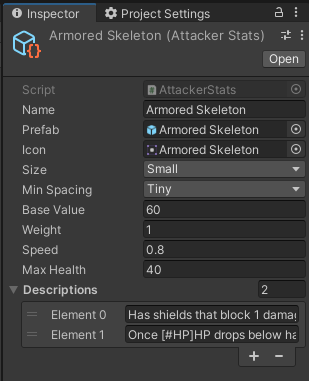
\includegraphics[width=\linewidth]{img/Steps/attacker stats inspector.png}}
    \end{tabular}
\end{flushleft}

\textbf{3.4.}
\emph{Base Value} denotes the attacker's value for the purposes of wave generation.
Attackers with higher value are considered more difficult to kill.
The value should be equal to \emph{Max Health} for attackers without abilities, and appropriately higher or lower if the attacker has some abilities.
This is further explained in section~\ref{sec:analysis-waves-abilities}.

\textbf{3.5.}
\emph{Weight} denotes how likely is this attacker to be selected when the wave generator decides between multiple attackers.
In the demo version, all attackers have weight 1.

\textbf{3.6.}
The \emph{Descriptions} array should contain human-readable description of the attacker's special abilities.
Each ability should be a separate entry.
Formatting tags can be used, as described in section~\ref{sec:analysis-description-tags}.
The implemented tags are summarized in section \xxx{TODO}.

\textbf{3.7.}
The \emph{Icon} represents the attacker in the incoming wave preview and the info panel.
The icons we use for attackers are placed in the asset folder \emph{Sprites/Icons/Attackers} and are $200\times200$ pixels in size.

\textbf{3.8.}
The \emph{Prefab} field contains the prefab of the attacker as it will exist in the game world.
It should contain the attacker's behavior and its 3D model with other visuals.
In the following subsection, we explain how to create this prefab.

\subsection{Attacker Prefab}

The attacker prefabs have many components in common, so we recommend copying an existing attacker prefab and editing it.
However, to explain all the components, in this section we'll create a new attacker prefab from scratch.
The prefabs of attackers are placed in the asset folder \emph{Prefabs/Attackers}.

\textbf{4.}
To create a new prefab, right-click in the folder and select \emph{Create > Prefab}.
We recommend giving it the same name as the attacker stats file.

\textbf{5.}
To the root game object of the prefab, attach the \mono{Attacker} script.
If the attacker requires more complex behavior, it can be achieved by either adding other scripts onto the attacker game object, or by using a script derived from \mono{Attacker} which implements this behavior.
For example, the \emph{Armored Skeleton} attacker has special abilities which are implemented in the \mono{ArmoredSkeleton} script.
Implementation of this script is described in section \xxx{TODO}.
This script has various settings and references which we'll fill out as we continue.

\begin{flushleft}
    \begin{tabular}{@{}>{\setlength\parindent{1em}}p{0.6\textwidth}p{\dimexpr 0.4\textwidth-2\tabcolsep}@{}}
        \textbf{6.}
        Next, attach a \emph{Rigidbody} script.
        Disable \emph{Use Gravity}, enable \emph{Is Kinematic} and set \emph{Collision Detection} to \emph{Continuous}.
        Finally, assign this component to the field \emph{Rb} in the \mono{Attacker} script.
         & \raisebox{\dimexpr -1\height+2mm}{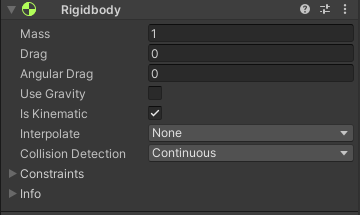
\includegraphics[width=\linewidth]{img/Steps/rigidbody inspector.png}}
    \end{tabular}
\end{flushleft}

\begin{flushleft}
    \begin{tabular}{@{}>{\setlength\parindent{1em}}p{0.6\textwidth}p{\dimexpr 0.4\textwidth-2\tabcolsep}@{}}
        \textbf{7.}
        Then, attach a collider that will be used for collision detection by projectiles.
        It should approximate the attacker's model, so once the attacker visuals are finalized, come back and tweak it.
        Additionally, make sure to set the \emph{Layer} of the attacker game object to \emph{Attacker}.
         & \centering\raisebox{\dimexpr -1\height+2mm}{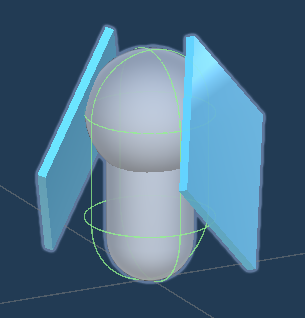
\includegraphics[width=0.7\linewidth]{img/Steps/attacker collider.png}}
    \end{tabular}
\end{flushleft}

\textbf{8.}
Next, attach the \mono{Selectable} script and assign the \mono{Attacker} script to its \emph{Attacker} field.

\textbf{9.}
The last script the attacker game object needs is a \mono{HighlightProvider} script.
The purpose of highlight providers is explained in section~\ref{sec:docs-highlights}.
For most attackers, the \mono{AttackerHighlightProvider}, which provides no additional highlights, is sufficient.
Example highlight provider implementation is described in section \xxx{TODO}.

\begin{flushleft}
    \begin{tabular}{@{}>{\setlength\parindent{1em}}p{0.6\textwidth}p{\dimexpr 0.4\textwidth-2\tabcolsep}@{}}
        \textbf{10.}
        Next, we add the target towers aim for.
        Create an empty game object as a child of the root game object.
        Set its \emph{Layer} to \emph{AttackerTarget}.
        Set its position to $(0, 0.15, 0)$ for small attackers and $(0, 0.3, 0)$ for large attackers.
        Then, attach a \emph{Sphere Collider} and set its radius to \mono{1e-05}.
        Finally, assign this object to the \emph{Target} field of the \mono{Attacker} script.
         & \centering\raisebox{\dimexpr -1\height+2mm}{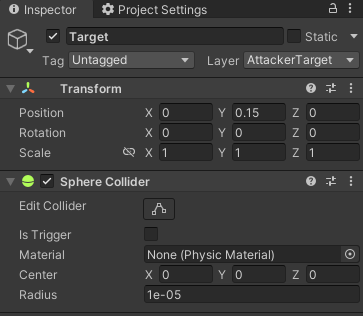
\includegraphics[width=\linewidth]{img/Steps/attacker target inspector.png}}
    \end{tabular}
\end{flushleft}

\textbf{11.}
Next, we'll set up all the visual parts of the attacker prefab.
Start by creating an empty child of the root object, which will be our root object for everything visual.
We will call it the visual root.
All visuals should go under one common root object, because we want them to move together.
However, they will move independently of the attacker prefab root object, because that one is moved 20 times per second by the \mono{Attacker} script.
This object's movement should be smooth, and for that, attach to it the \mono{PositionInterpolation} script, and assign the attacker root object to its \emph{Sim} field.

\textbf{12.}
Now it's a good time to add the attacker model, and other custom visuals.
Our models are composed of primitive shapes, and they aren't animated, though some attackers have particle effects.
The only restrictions here are that the target the towers are going to aim for should be within the attacker's body.
After this, we can go back and adjust the root collider to match the model.

\textbf{13.}
Next, we add an empty child object under the visual root, which will be the visual target.
Its position should match the attacker target~--- $(0, 0.15, 0)$ for small attackers and $(0, 0.3, 0)$ for large attackers~--- but it will move smoothly with the rest of the visuals.
It is used by towers to visually aim at the apparent location of the attacker, without jumping 20 times per second.
To fulfill this role, assign the object to the \emph{Visual Target} field of the \mono{Attacker} script.

\begin{flushleft}
    \begin{tabular}{@{}>{\setlength\parindent{1em}}p{0.6\textwidth}p{\dimexpr 0.4\textwidth-2\tabcolsep}@{}}
        \textbf{14.}
        Then, we add the collider, which is used to let the player select the attacker.
        For that, create another object under the visual root and give it a collider.
        Again, try to match the attacker model, but a slightly bigger collider is better, so the attacker is easier to select.
        Finally, set the layer of this object to \emph{SelectionAttacker}.
        In the figure on the right we show the attacker collider along with the bigger selection collider.
         & \centering\raisebox{\dimexpr -1\height+2mm}{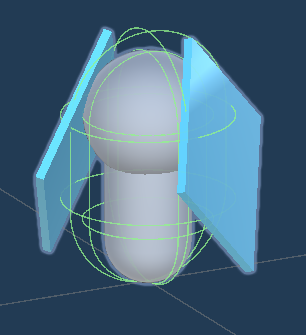
\includegraphics[width=0.7\linewidth]{img/Steps/attacker selection.png}}
    \end{tabular}
\end{flushleft}

\begin{flushleft}
    \begin{tabular}{@{}>{\setlength\parindent{1em}}p{0.6\textwidth}p{\dimexpr 0.4\textwidth-2\tabcolsep}@{}}
        \textbf{15.}
        Next, we add attacker's health display.
        For that, place the prefab \emph{HealthCanvas} under the visual root.
        Position it at the top of the attacker model as shown in the figure on the right.
        The health display graphic will hover slightly above the attacker model.
        Then, go to the child object \emph{Health} and assign the attacker root object to the \emph{Attacker} field of its \mono{HealthDisplay} script.
         & \centering\raisebox{\dimexpr -1\height+2mm}{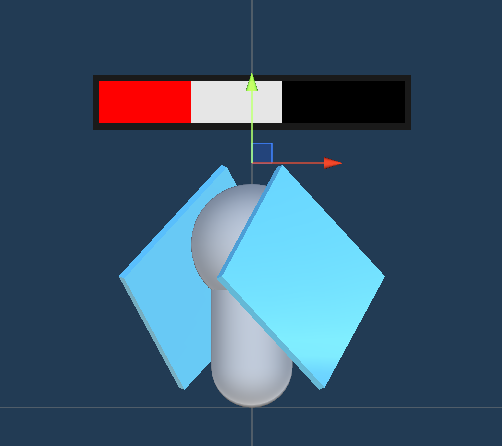
\includegraphics[width=\linewidth]{img/Steps/health display.png}}
    \end{tabular}
\end{flushleft}

\begin{flushleft}
    \begin{tabular}{@{}>{\setlength\parindent{1em}}p{0.6\textwidth}p{\dimexpr 0.4\textwidth-2\tabcolsep}@{}}
        \textbf{16.}
        Now we also add attacker's highlight.
        Place the prefab \emph{HighlightCanvas} under the visual root.
        Position it in the center of the attacker model.

        Then, go to the child object \emph{Highlight} and adjust it.
        Make the color of its \emph{Image} fully opaque to see what the highlight will look like.
        Adjust the \emph{Highlight} scale so that the highlight creates an outline around the attacker model.
        It should look similar to the one shown in the figure on the right.
        Don't forget to turn the opacity back to 0 when finished.

        Finally, assign a reference to the \emph{Highlight} object to the fields \emph{Highlight} and \emph{Highlight Anim} in the \mono{Attacker} script.
         & \centering\raisebox{\dimexpr -1\height+2mm}{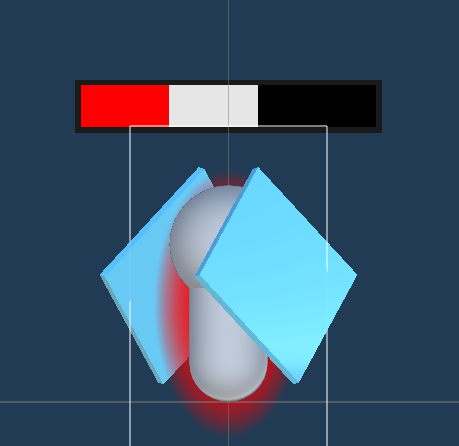
\includegraphics[width=\linewidth]{img/Steps/attacker highlight.png}}
    \end{tabular}
\end{flushleft}

\begin{flushleft}
    \begin{tabular}{@{}>{\setlength\parindent{1em}}p{0.6\textwidth}p{\dimexpr 0.4\textwidth-2\tabcolsep}@{}}
        \textbf{17.}
        As the last step, we assign some reactions to events the \mono{Attacker} script provides.
        For example, we should subscribe some death animation to the \emph{On Death} event.
        As shown in the figure on the right, in our current implementation, we only deactivate the game object that holds the attacker's model, deactivate its health display, and we play a particle effect.
         & \centering\raisebox{\dimexpr -1\height+2mm}{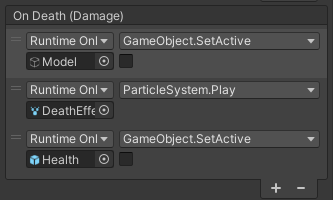
\includegraphics[width=\linewidth]{img/Steps/attacker events.png}}
    \end{tabular}
\end{flushleft}

\subsection{Attacker Behavior Script Example}

In this section we describe how is the \emph{Armored Skeleton} attacker behavior script implemented.
The source code is for reference shown as code snippet~\ref{code:armored-skeleton}, but we've omitted the usings and namespace definition to save space.

As we can see, the class extends the \mono{Attacker} script.
This attacker has two special abilities:
\enquote{Has shields that block 1 damage from each hit.
    Once HP drops below half of max HP, loses the shields and doubles its speed.}
For this we've added a setting \mono{damageReduction} to configure by how much the shields reduce the incoming damage.
And a Unity event, that will let the attacker visuals react, and hide the shields from the model once the attacker loses them.
The field \mono{hasShield} just remembers the state.
This is tracked explicitly, so the shields don't come back up when the attacker heals back from below half HP.

\begin{listing}[H]
    \begin{minted}{csharp}
public class ArmoredSkeleton : Attacker
{
    [SerializeField] int damageReduction;
    [SerializeField] UnityEvent onShieldDropped;
    [SerializeField] bool hasShield;

    static ArmoredSkeleton()
    {
        DAMAGE.RegisterModifier(TryBlockDamage, -1);
        DAMAGE.RegisterReaction(OnDamaged, 1000);
        SPEED.RegisterModifier(UpdateSpeed, -1000000);
    }

    static bool TryBlockDamage(ref (Attacker target, Damage damage) param)
    {
        if (param.target is not ArmoredSkeleton { hasShield: true } s ||
            param.damage.type.HasFlag(Damage.Type.HealthLoss))
            return true;

        param.damage.amount -= s.damageReduction;
        return param.damage.amount > 0;
    }

    static void OnDamaged((Attacker target, Damage damage) param)
    {
        if (param.target is not ArmoredSkeleton { hasShield: true } s ||
            s.health >= (s.stats.maxHealth + 1) / 2)
            return;

        s.hasShield = false;
        s.onShieldDropped.Invoke();
    }

    static void UpdateSpeed(Attacker attacker, ref float speed)
    {
        if (attacker is ArmoredSkeleton { hasShield: false })
            speed *= 2;
    }
}
    \end{minted}
    \caption{\mono{ArmoredSkeleton} behavior script implementation.}
    \label{code:armored-skeleton}
\end{listing}

The \emph{Armored Skeleton} abilities modify how much damage they take and their speed.
To do this, we register modifiers to the modifiable command \mono{DAMAGE} and query \mono{SPEED}.
Because both of them are static, and the attacker is provided as an argument to the modifier methods, we modify them using static methods, registered in the \mono{ArmoredSkeleton} static constructor.
We also register a reaction to damage in order to check the attacker's HP whenever it is damaged.
The number provided as a second argument to the register methods is just the priority.

The command \mono{DAMAGE} is modified by the \mono{TryBlockDamage} method.
It checks whether the damaged attacker is an armored skeleton with its shields still up, and that the damage isn't of type \mono{HealthLoss}, which ignores all damage modifiers.
Then it reduces the damage by the attacker's \mono{damageReduction}.
If the damage becomes 0 or less, we return \mono{false} to completely block the damage command.

Whenever any attacker takes damage, the \mono{OnDamaged} event is notified.
It checks whether the attacker is an \mono{ArmoredSkeleton} with shields.
If it is, and its new HP is below half of max HP, it makes it drop its shield.
Finally, the attacker's speed is modified by the \mono{UpdateSpeed} method, which just doubles the speed value, if the attacker is an \mono{ArmoredSkeleton} with its shields gone.

\section{Blueprints}

- scriptable object

- abilities

- example script

- buildings

- towers

- example script

- placement example script

- highlights example script

- description tags

\section{Terrain Types}\label{sec:docs-terrain-type}

In this section, we explain how to add a new terrain type to the game.
Terrain types are automatically loaded from the asset folder \emph{StreamingAssets/TerrainTypes}.
Each terrain type has to be a file with the \mono{.txt} extension.
The terrain type a world should use is set in the \mono{WorldSettings} script in the field \emph{Terrain Type}.
Currently, it is set to the terrain type \emph{Test}.
To automatically select different terrain types for different levels, the \mono{LevelSetter} script needs to be modified to implement this behavior.
\mono{LevelSetter} is the script that automatically sets up world settings for each level, as described in section~\ref{sec:docs-level-init}.

In the rest of this section we describe the structure of the terrain type file format.
To understand the properties it contains, we recommend first reading sections~\ref{sec:analysis-terrain-generation} and~\ref{sec:analysis-obstacles}.

\subsection{General Syntax}

The terrain type files use custom syntax that was designed to encode structured information, but is human-readable and human-writable.

\head{Whitespace and Comments}{}
Line breaks often matter, but otherwise all strings of whitespace are equivalent.
All indentation is purely for readability purposes.
One line comments are created using the \mono{\#}~character, meaning that it and all characters following it are treated as whitespace, until the end of the line.
The \mono{\%}~character is used to create multiline comments.
Everything between two \mono{\%}~characters is treated as whitespace.

\head{Overall Structure}
The file is composed of several top-level properties.
Each property consists of a name, followed by its value.
The properties can be defined in any order, but we place them in a specific order to improve readability.
The file contains several one-line properties, and three block properties:
\begin{minted}{text}
display_name ...
free_surfaces ...
blocked_surfaces ...
free_edges ...
blocked_edges ...
max_height ...

modules { ... }
obstacles { ... }
scatterer { ... }
\end{minted}

We will explain the one-line properties in the following subsection, and each block property will be explained in its own subsection after that.
We would also like to note that \emph{string} values are not enclosed in quotation marks, and they cannot contain whitespace.

\subsection{One-Line Top Level Properties}

\head{\mono{display\_name <name>}}{}
The name by which this terrain type is identified.\\
\textbf{name}: A string.

\head{\mono{free\_surfaces <keys>}}{}
Defines which surface types used by this terrain type's modules are free.
Each surface type is represented by a single uppercase letter.
Obstacles and buildings can be placed on free surfaces, and paths can go over them.\\
\textbf{keys}: A string composed of uppercase letters. Each letter is one surface type.

\head{\mono{blocked\_surfaces <keys>}}{}
\emph{optional}\\
Defines which surface types used by this terrain type's modules are blocked.
Each surface type is represented by a single uppercase letter.
Obstacles and buildings cannot be placed on blocked surfaces, and paths cannot go over them.\\
\textbf{keys}: A string composed of uppercase letters. Each letter is one surface type.\\
Default value: \emph{none}.

\head{\mono{free\_edges <keys>}}{}
Defines which edge types used by this terrain type's modules are free.
Each edge type is represented by a single uppercase letter.
Paths can go through free edges.\\
\textbf{keys}: A string composed of uppercase letters. Each letter is one edge type.

\head{\mono{blocked\_edges <keys>}}{}
\emph{optional}\\
Defines which edge types used by this terrain type's modules are blocked.
Each edge type is represented by a single uppercase letter.
Paths cannot go through blocked edges.\\
\textbf{keys}: A string composed of uppercase letters. Each letter is one edge type.\\
Default value: \emph{none}.

\head{\mono{max\_height <value>}}{}
Maximum terrain height level.
The minimum height level is 0, so the total number of height levels is $\mono{value} + 1$.\\
\textbf{value}: A non-negative integer.

\subsection{Modules}

The \mono{modules} property defines the list of terrain modules to be used for terrain generation.
Each module is denoted by a \mono{*}~character followed by the module name and a block containing its properties.

\begin{minted}{text}
modules {
    * <ModuleName> {
        weight ...
        variants ...
        height_offset ...
        collision ...
        shape { ... }
        heights ...
    }
    ...
}
\end{minted}

\head{\mono{weight <value>}}{}
How likely is this module to be selected when collapsing a slot.\\
\textbf{value}: A positive floating-point number.

\head{\mono{variants <flags>}}{}
\emph{optional}\\
Which symmetric variants of this module can the terrain generator use.\\
\textbf{flags}: \mono{0}, \mono{2} or \mono{4} to denote the number of rotational symmetries, and optionally \mono{f} or \mono{F} to denote reflection.
For example, the code \mono{f4} means this module can be freely flipped and rotated.\\
Default value: \mono{0}.

\head{\mono{height\_offset <value>}}{}
\emph{optional}\\
Determines the height offset of the module mesh.
Positive values mean the mesh is placed higher than the module's height level, negative values mean lower.\\
\textbf{value}: A floating-point number.\\
Default value: \mono{0}.

\head{\mono{collision <path>}}{}
The collision mesh of the module.\\
\textbf{path}: The path to the mesh, relative to the asset folder \emph{Models/Resources}. Must not contain file extension.

\head{\mono{shape}}{}
The shape of this module.
Basically, the edge and corner constraints this module imposes on adjacent slots, as shown in figure~\ref{fig:wfc-module-2}.
The values are placed in a square to visually convey the direction they are tied to, however, they would still be parsed correctly even when placed on one line.
\begin{minted}{text}
shape {
    <surface><height><slant> <edge> <surface><height><slant>
              <edge>                          <edge>
    <surface><height><slant> <edge> <surface><height><slant>
}
\end{minted}
\textbf{surface}: Uppercase letter representing a surface type.\\
\textbf{height}: A digit representing the height level, relative to the module's lowest height level.\\
\textbf{slant}: Direction of the tile slant~--- \mono{\^}, \mono{v}, \mono{<}, \mono{>} for north, south, west, east, or \mono{x} for no slant.\\
\textbf{edge}: Uppercase letter representing an edge type.

\head{\mono{heights <digits>}}{}
\emph{optional}\\
Defines the height levels this module can be at.\\
\textbf{digits}: A sequence of digits, each representing one valid height.\\
Default value: All heights from \mono{0} to \mono{max\_height}.

\head{Example Module}{}
This is the definition of the module shown in figure~\ref{fig:wfc-module-2}.
\begin{minted}{text}
* CornerCliffSlantUp {
    weight 32
    variants f4
    collision Terrain/CornerSlantUp
    height_offset 1
    shape {
        D1x X D1v
         X     O
        D0x O D0x
    }
}
\end{minted}

\begin{center}
    \captionsetup{type=figure}
    \begin{minipage}{.5\textwidth}
        \centering
        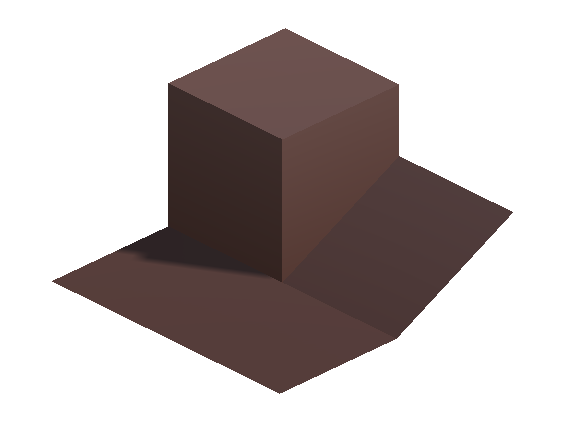
\includegraphics[width=0.95\textwidth]{img/Module model.png}
        \subcaption{The 3D geometry of the module.}
    \end{minipage}%
    \begin{minipage}{.5\textwidth}
        \centering
        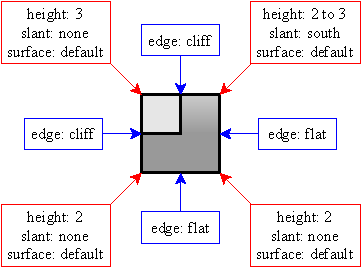
\includegraphics[width=0.95\textwidth]{img/Module constraints.pdf}
        \subcaption{A view from above with the constraints.}
    \end{minipage}
    \caption{An example module and its constraints (copy).}
    \label{fig:wfc-module-2}
\end{center}

\subsection{Obstacles}

The \mono{obstacles} property contains obstacle definitions and properties that determine their placement, as described in section~\ref{sec:analysis-obstacles}.
The block contains one named property \mono{phases}, and the individual obstacle definitions.
Each obstacle is denoted by a \mono{*}~character, followed by its name and block with its properties.

\begin{minted}{text}
obstacles {
    phases {
        <Phase1>
        <Phase2>
        ...
    }

    * <ObstacleName> {
        type ...
        min ...
        max ...
        base_probability ...
        valid_surfaces ...
        on_slants ...
        affinities ...
    }
    ...
}
\end{minted}

\head{\mono{phases}}
Define which obstacles are placed in which phase.
Each line represents one phase, and it consists of the names of the obstacles to be place, separated by whitespace: \mono{<Obstacle1> <Obstacle2> ...}.

\head{\mono{type <type>}}{}
Defines the obstacle type~--- one of \emph{large}, \emph{small}, \emph{small fuel-rich} and \mono{small mineral-rich}.\\
\textbf{type}: One of strings: \mono{l}, \mono{large}, \mono{s}, \mono{small}, \mono{f}, \mono{fuel}, \mono{m} or \mono{minerals}.

\head{\mono{min <value>}}{}
\emph{optional}\\
Minimum number of tiles with this obstacle.\\
\textbf{value}: A non-negative integer, less than or equal to \mono{max}.\\
Default value: \mono{0}.

\head{\mono{max <value>}}{}
\emph{optional}\\
Maximum number of tiles with this obstacle.\\
\textbf{value}: A non-negative integer, more than or equal to \mono{max}.\\
Default value: \emph{no limit}.

\head{\mono{base\_probability <value>}}{}
Base probability to place this obstacle for each tile.\\
\textbf{value}: A floating-point number.

\head{\mono{valid\_surfaces <keys>}}{}
\emph{optional}\\
The surface types this obstacle can be placed on.\\
\textbf{keys}: A string composed of uppercase letters. Each letter is one surface type.\\
Default value: \emph{all surfaces}.

\head{\mono{on\_slants <bool>}}{}
\emph{optional}\\
Determines whether this obstacle can be placed on a slanted tile.\\
\textbf{bool}: \mono{true} or \mono{false}.\\
Default value: \mono{true}.

\head{\mono{affinities <entry1> <entry2> ...}}{}
The affinity for each layer.
Affinity greater than zero means the probability to place the obstacle increases with proximity to obstacle placed in the given layer.
Analogously, negative affinity decreases the probability.\\
Each entry is a floating-point number, and is assumed to be \mono{0} for layers for which it wasn't specified.

\head{Obstacle Definition Example}{}
\begin{minted}{text}
* Minerals {
    type m
    min 6
    max 8
    base_probability 0.3
    on_slants false
    affinities -1.5 0.3
}
\end{minted}

\subsection{Scatterer}

The \mono{scatterer} property defines how obstacle models are placed on the generated terrain, as described in section~\ref{sec:analysis-obstacle-models}.
It is a list of the model placement definitions, each denoted by a \mono{*}~character followed by a name and a block containing its properties.

\begin{minted}{text}
scatterer {
    * <ModelName> {
        prefab ...
        tries_per_tile ...
        placement_radius ...
        persistent_radius ...
        size_gain ...
        radius_gain ...
        angle_spread ...
        value_threshold ...
        value { ... }
    }
}
\end{minted}

\head{\mono{prefab <path>}}{}
The prefab to be instantiated.\\
\textbf{path}: The path to the prefab, relative to the asset folder \emph{Prefabs/Resources}. Must not contain file extension.

\head{\mono{tries\_per\_tile <value>}}{}
Number of attempts to place the model per tile.\\
\textbf{value}: A positive integer.

\head{\mono{placement\_radius <value>}}{}
The base radius to check for collision with already placed models.\\
\textbf{value}: A non-negative floating-point number.

\head{\mono{persistent\_radius <value>}}{}
The base radius of the collision the model will have once placed, used for collision checks for models placed after it.\\
\textbf{value}: A non-negative floating-point number.

\head{\mono{size\_gain <value>}}{}
The proportion at which the scale of the placed model increases or decreases based on the noise expression value at the placement point.
For example with \mono{size\_gain 1}, a model placed at point with noise expression value 1 will have scale 2, and at point with value -2, it will have scale 1/3.\\
\textbf{value}: A floating-point number.

\head{\mono{radius\_gain <value>}}{}
The proportion at which the scale of the model radius increases or decreases based on the noise expression value at the placement point.
For example with \mono{redius\_gain -1}, a model placed at point with noise expression value 1 will have its \mono{placement\_radius} and \mono{persistent\_radius} halved.\\
\textbf{value}: A floating-point number.

\head{\mono{angle\_spread <value>}}{}
By how big of an angle can the placed model be randomly tilted.\\
\textbf{value}: A non-negative floating-point number representing the angle in degrees.

\head{\mono{value\_threshold <value>}}{}
The model cannot be placed at points with noise expression value less than the threshold.\\
\textbf{value}: A floating-point number.

\head{\mono{value <noise\_expression\_nodes>}}{}
The noise expression that determines the value for this model at any given point.
The expression is the sum of the expressions provided as the argument.

\head{\mono{noise\_expression\_nodes}}{}
A block with one or more \mono{noise\_expression\_node} entries, separated by whitespace (including line breaks): \mono{\{ <node1> <node2> ... \}}.

\head{\mono{noise\_expression\_node}}{}
One of \mono{<const>}, \mono{<sum>}, \mono{<mult>}, \mono{<clamp>}, \mono{<path>}, \mono{<path>}, \mono{<obstacle>}, \mono{<height>}, or \mono{<fractal\_noise>}.

\head{\mono{const <value>}}{}
Has a constant value at every point.\\
\textbf{value}: A floating-point number.

\head{\mono{sum <noise\_expression\_nodes>}}{}
Returns the sum of the subexpressions.

\head{\mono{mult <multiplier> <noise\_expression\_nodes>}}{}
Returns the sum of the subexpressions multiplied by the \mono{multiplier}.\\
\textbf{multiplier}: A floating-point number.

\head{\mono{clamp <min> <max> <noise\_expression\_nodes>}}{}
Returns the sum of the subexpressions, but clamped to be between \mono{min} and \mono{max}.\\
\textbf{min}: A floating-point number.\\
\textbf{max}: A floating-point number.

\head{\mono{path <in> <out>}}{}
Returns the signed distance function to the tiles containing a path.
The parameters \mono{in} and \mono{out} specify the sign and magnitude of the value inside and outside the tiles with path.\\
\textbf{in}: A floating-point number.\\
\textbf{out}: A floating-point number.

\head{\mono{obstacle <ObstacleName> <in> <out>}}{}
Returns the signed distance function to the tiles containing the specified obstacle.
The parameters \mono{in} and \mono{out} specify the sign and magnitude of the value inside and outside the tiles with the obstacle.\\
\textbf{ObstacleName}: Name of the obstacle.\\
\textbf{in}: A floating-point number.\\
\textbf{out}: A floating-point number.

\head{\mono{height}}{}
Returns the terrain height level at the given point, including fractional values on slopes.

\head{\mono{fractal\_noise <properties>}}{}
Returns a value generated by summing several layers of Perlin noise.\\
\textbf{properties}: A block with the following named properties:
\begin{minted}{text}
fractal_noise {
    octaves ...
    bias ...
    base_amplitude ...
    amplitude_mult ...
    base_frequency ...
    frequency_mult ...
}
\end{minted}

\head{\mono{octaves <value>}}{}
The number of noise layers.\\
\textbf{value}: A positive integer.

\head{\mono{bias <value>}}{}
A constant value added to each point.\\
\textbf{value}: A floating-point number.

\head{\mono{base\_amplitude <value>}}{}
The amplitude of the first noise layer.
For example, noise with amplitude 2 produces values between -2 and 2.\\
\textbf{value}: A floating-point number.

\head{\mono{amplitude\_mult <value>}}{}
Each noise layer's amplitude is the amplitude of the previous layer multiplied by this value.\\
\textbf{value}: A positive floating-point number.

\head{\mono{base\_frequency <value>}}{}
The frequency of the first noise layer, in other words, the reciprocal of its scale.\\
\textbf{value}: A floating-point number.

\head{\mono{frequency\_mult <value>}}{}
Each noise layer's frequency is the frequency of the previous layer multiplied by this value.\\
\textbf{value}: A positive floating-point number.

\head{Obstacle Model Placement Example}{}
\begin{minted}{text}
* Minerals {
    prefab Terrain/obstacles/Minerals
    tries_per_tile 50
    placement_radius 0.05
    persistent_radius 0.15
    size_gain 2
    radius_gain -0.5
    angle_spread 25
    value_threshold 0
    value {
        clamp -3 0.7 {
            obstacle Minerals 1 -1
            fractal_noise {
                octaves 2
                bias 0
                base_amplitude 0.3
                amplitude_mult 0.777
                base_frequency 0.61
                frequency_mult 2.137
            }
            path -3 0
        }
    }
}
\end{minted}
